\documentclass[10pt,twocolumn,letterpaper]{article}
\usepackage[top=0.75in,bottom=0.75in,left=0.75in,right=0.75in]{geometry}
\usepackage{booktabs}
\usepackage{graphicx}
\usepackage{hyperref}
\usepackage{parskip}
\usepackage{titlesec}
%\usepackage{microtype}
\usepackage{enumitem}
\setlist{nosep, leftmargin=1.2em}
\hypersetup{colorlinks=true, urlcolor=blue, linkcolor=blue}

\titleformat{\section}{\normalsize\bfseries\scshape}{}{0em}{}[\vspace{-0.3em}\hrule\vspace{0.2em}]
\titleformat{\subsection}{\small\bfseries}{}{0em}{}
\titlespacing{\section}{0pt}{6pt}{2pt}
\titlespacing{\subsection}{0pt}{4pt}{1pt}

\setlength{\columnsep}{0.25in}
\setlength{\parskip}{3pt}

\begin{document}

\twocolumn[{%
\begin{center}
  {\large\bfseries Mapping \& Analyzing Participation in Tutor/Mentor\\
  Leadership and Networking Conferences}\\[4pt]
  {\small Brian Hanley, Matthew Guschwan, Timothy Kelley, Patrick Green\\
  Indiana University, Luddy School of Informatics, Computing, and Engineering}
\end{center}
\vspace{4pt}
}]

%-----------------------------------------------------------------------
\section{Introduction and Prior Work}

The primary deliverable of this project is a \textbf{repeatable,
deployable data-to-visualization pipeline} for conference participation
analysis. The pipeline ingests a standardized CSV, normalizes
organizational categories, computes network structures, and serves
live JSON exports that any visualization tool---Kumu.io, Gephi, or a
browser-based library---can consume directly. The
Tutor/Mentor Conference dataset is the demonstration case; the
pipeline is designed to work with any conference dataset that follows
the same schema, as realized in the companion
\textit{YourConferenceNetwork} application.

This phase builds on Fall~2025 student teams~\cite{teamk2025} who
produced an open-source Kumu.io template from the same data. Our
contribution is the step from static template to live, maintainable
system: persistent storage, queryable API endpoints, and an explicit
handoff design so future teams can extend rather than restart.
The live deployment is at
\href{https://tutormentor.brianhanley.dev}{tutormentor.brianhanley.dev}.

\subsection{Stakeholder Groups}

Four stakeholder groups guided design. (1)~\textbf{Project sponsor}:
Daniel F.\ Bassill (Tutor/Mentor Connection, 1993--2011;
Tutor/Mentor Institute LLC, 2011--present)~\cite{bassill2025}, who
needs a publicly shareable visualization of 21 years of network history.
(2)~\textbf{Conference participants and their organizations}---youth-serving
nonprofits, businesses, colleges, K--12 schools, government agencies,
faith communities, and foundations---who benefit from accurate, linked
records of their historical involvement.
(3)~\textbf{Researchers and civic advocates} who require a
reproducible, documented dataset for further analysis.
(4)~\textbf{General public and prospective partners} visiting
\href{https://tutormentorexchange.net}{tutormentorexchange.net} who
need an intuitive entry point into the network.

\subsection{Stakeholder Needs}

Bassill requires color-coded nodes by organization type, organization
search, and hyperlinks to current websites. Participants need
accurate categorization and active website links. Researchers need
structured, documented exports. Across all groups the shared need is
for a tool that is publicly accessible, clearly navigable, and
maintainable across semesters.

%-----------------------------------------------------------------------
\section{Data Acquisition}

\subsection{Data Sources}

The primary source is the cleaned participation spreadsheet prepared
by Fall~2025 TeamK~\cite{teamk2025} (updated February~11,~2026),
covering May~1994 through November~2014. A secondary source is the
\href{https://tutormentorexchange.net}{tutormentorexchange.net}
program directory, supplemented by an automated DuckDuckGo
crawler with archive.org fallback for locating organizational
websites~\cite{crawler2026}.

\subsection{Data Description, Quality, and Coverage}

The dataset contains \textbf{6,410} participation records across
18 columns and \textbf{41 conference events}. Each record represents
one individual's attendance and includes: UniqueID, Salutation,
First/Last Name, SNA Category (original and cleaned), Title (original
and cleaned), Organization (original and cleaned), Active/Inactive
status, Address, City, State, Zip, Conference, Month, and Year.

Geographic coverage is predominantly Chicago (IL: 5,305 of
state-coded records; IN:~97; WI:~93). \textbf{270 records (4.2\%)}
have a blank organization field; these are excluded from all network
exports and edge-list analytics but retained in the database.
Additional quality notes:
\begin{itemize}
  \item The \texttt{active\_inactive} column is inconsistently populated
        and was excluded from analysis.
  \item Address/ZIP fields are sparsely populated for pre-2000 records.
  \item Organization names change across decades; cross-decade queries
        may miss the same entity under a variant name.
  \item Individuals who moved between organizations appear as separate
        org records rather than a single person with multiple affiliations.
  \item The dataset ends in 2014; the network reflects a historical
        snapshot, not current activity.
\end{itemize}

%-----------------------------------------------------------------------
\section{Analysis Pipeline}

The pipeline follows four sequential stages (Table~\ref{tab:pipeline}).
Each stage produces a well-defined output that feeds the next, making
the full workflow reproducible by any team that starts from the same
CSV schema.

\begin{table}[t]
\small
\caption{Pipeline stages and primary outputs.}
\label{tab:pipeline}
\begin{tabular}{lp{4.5cm}}
\toprule
Stage & Output \\
\midrule
1.\ Ingest \& Normalize & Loaded \texttt{Attendance} table; 69 raw SNA variants → 12 canonical categories \\
2.\ Participation Analysis & Year/sector/state attendance aggregates served at \texttt{/chart/} \\
3.\ URL Enrichment & \texttt{org\_websites.csv}: live, archived, unverified, not found status per org \\
4.\ Network Export & 4 live JSON/CSV endpoints at \texttt{/export/} for Kumu.io and Gephi \\
\bottomrule
\end{tabular}
\end{table}

\subsection{Stage 1 — Ingest and Normalize}

The \texttt{load\_data} management command reads the source CSV,
applies \texttt{conferences/sna\_normalize.py}, and populates the
\texttt{Attendance} table. The normalization map resolves 69 raw
spelling and casing variants to 12 canonical SNA categories
(Table~\ref{tab:sna}), including \textbf{Media}---confirmed by Bassill
on April~22,~2026 and added in this submission. Re-running
\texttt{load\_data} with a revised CSV rebuilds the table without
duplicating records. Media's low representation in the current dataset
is itself a meaningful finding: journalists and communications
organizations are absent from a network where visibility is
a core strategic goal.

\begin{table}[t]
\small
\caption{SNA category distribution (6,410 records, database-verified).
  Media confirmed as 12th canonical category by D.F.\ Bassill, April~22,~2026.}
\label{tab:sna}
\begin{tabular}{lrr}
\toprule
Category & Records & \% \\
\midrule
Program      & 3,310 & 51.6 \\
Resource     &   612 &  9.5 \\
Other        &   529 &  8.3 \\
College      &   559 &  8.7 \\
K-12 School  &   418 &  6.5 \\
T/MC         &   239 &  3.7 \\
Intermediary &   227 &  3.5 \\
Faith        &   148 &  2.3 \\
Government   &   136 &  2.1 \\
Business     &   131 &  2.0 \\
Foundation   &    58 &  0.9 \\
Media        &    43 &  0.7 \\
\midrule
\textit{Blank org (excluded)} & \textit{270} & \textit{4.2} \\
\bottomrule
\end{tabular}
\end{table}

\subsection{Stage 2 — Participation Frequency Analysis}

Django ORM aggregations compute year-level attendance counts
segmented by SNA category. The resulting Plotly chart
(Fig.~\ref{fig:chart}) is interactive: filters by year, sector, and
state allow each stakeholder group to focus the view on the slice
most relevant to them. This single interface serves all four groups
simultaneously.

\subsection{Stage 3 — Organization URL Enrichment}

\texttt{find\_org\_websites.py} issued DuckDuckGo queries for each
of the 2,163 unique organizations, with archive.org fallback for
defunct sites. Each URL was verified with a live HTTP check.
Results in \texttt{org\_websites.csv} carry a status of
\texttt{live}, \texttt{archived}, \texttt{unverified}, or
\texttt{not found}. Roughly one quarter remain \texttt{unverified}
or \texttt{not found} and require manual review against the
\href{https://tutormentorexchange.net}{tutormentorexchange.net}
directory.

\subsection{Stage 4 — Network Structure and Export}

NetworkX structures the dataset into three graph models, each
answering a distinct analytical question:
\begin{itemize}
  \item \textbf{Org-event bipartite}: which organizations attended which events?
  \item \textbf{Org-org co-attendance} (Fig.~\ref{fig:network}): which
        organizations share conference history? Edge weight = number of
        conferences co-attended; node size = total event count.
  \item \textbf{Event-sector-org three-layer}: how do sectors cluster across the
        full conference timeline?
\end{itemize}

Four live endpoints at \texttt{/export/} (JSON and CSV) allow Kumu.io
to link maps directly to the running app, so maps update automatically
when the underlying data changes.

\subsection{Framework and Tool Justification}

Django was chosen over a standalone script or Jupyter notebook for
three reasons specific to this project's goals: (1)~persistent,
queryable storage that survives CSV re-imports without manual
intervention; (2)~live HTTP endpoints required by Kumu.io's
remote-JSON import feature; and (3)~a maintainable web application
that future teams can extend without rebuilding from scratch. Basic
Git proficiency (\texttt{add}/\texttt{commit}/\texttt{push}) is the
only prerequisite for contributing; deployment details are in the
project README.

%-----------------------------------------------------------------------
\section{Visualizations}

\subsection{Participation Frequency Chart}

\begin{figure}[t]
  \centering
  % !!!!!!!!!!!!!!!!!!!!!!!!!!!!!!!!!!!!!!!!!!!!!!!!!!!!!!!!!!!!!!
  % REQUIRED BEFORE SUBMISSION: replace \fbox below with:
  %   \includegraphics[width=\columnwidth]{chart_screenshot.png}
  % Take screenshot from https://tutormentor.brianhanley.dev/chart/
  % Save as chart_screenshot.png in the same folder as this .tex file.
  % !!!!!!!!!!!!!!!!!!!!!!!!!!!!!!!!!!!!!!!!!!!!!!!!!!!!!!!!!!!!!!
  \fbox{\parbox{0.85\columnwidth}{\centering\vspace{1.5em}
    \small\textit{[Screenshot of Plotly chart at \texttt{/chart/}\\
    — replace before submission]}
  \vspace{1.5em}}}
  \caption{Participation frequency by year and SNA category (Plotly).
    Filters by year, sector, and state serve all four stakeholder groups
    from a single interface.}
  \label{fig:chart}
\end{figure}

The Plotly chart (Fig.~\ref{fig:chart}) reveals the full 1994--2014
arc: growth to a peak cluster in 1998--2001 and a sharp post-2009
decline. Interactive year/sector/state filters let Bassill focus on
specific outreach gaps and allow researchers to slice the data without
writing code. \textbf{Rebuilding to even half of peak attendance
(280+ per year) is a concrete, measurable goal} the chart makes
immediately visible.

\subsection{Org-Org Co-attendance Network}

\begin{figure}[t]
  \centering
  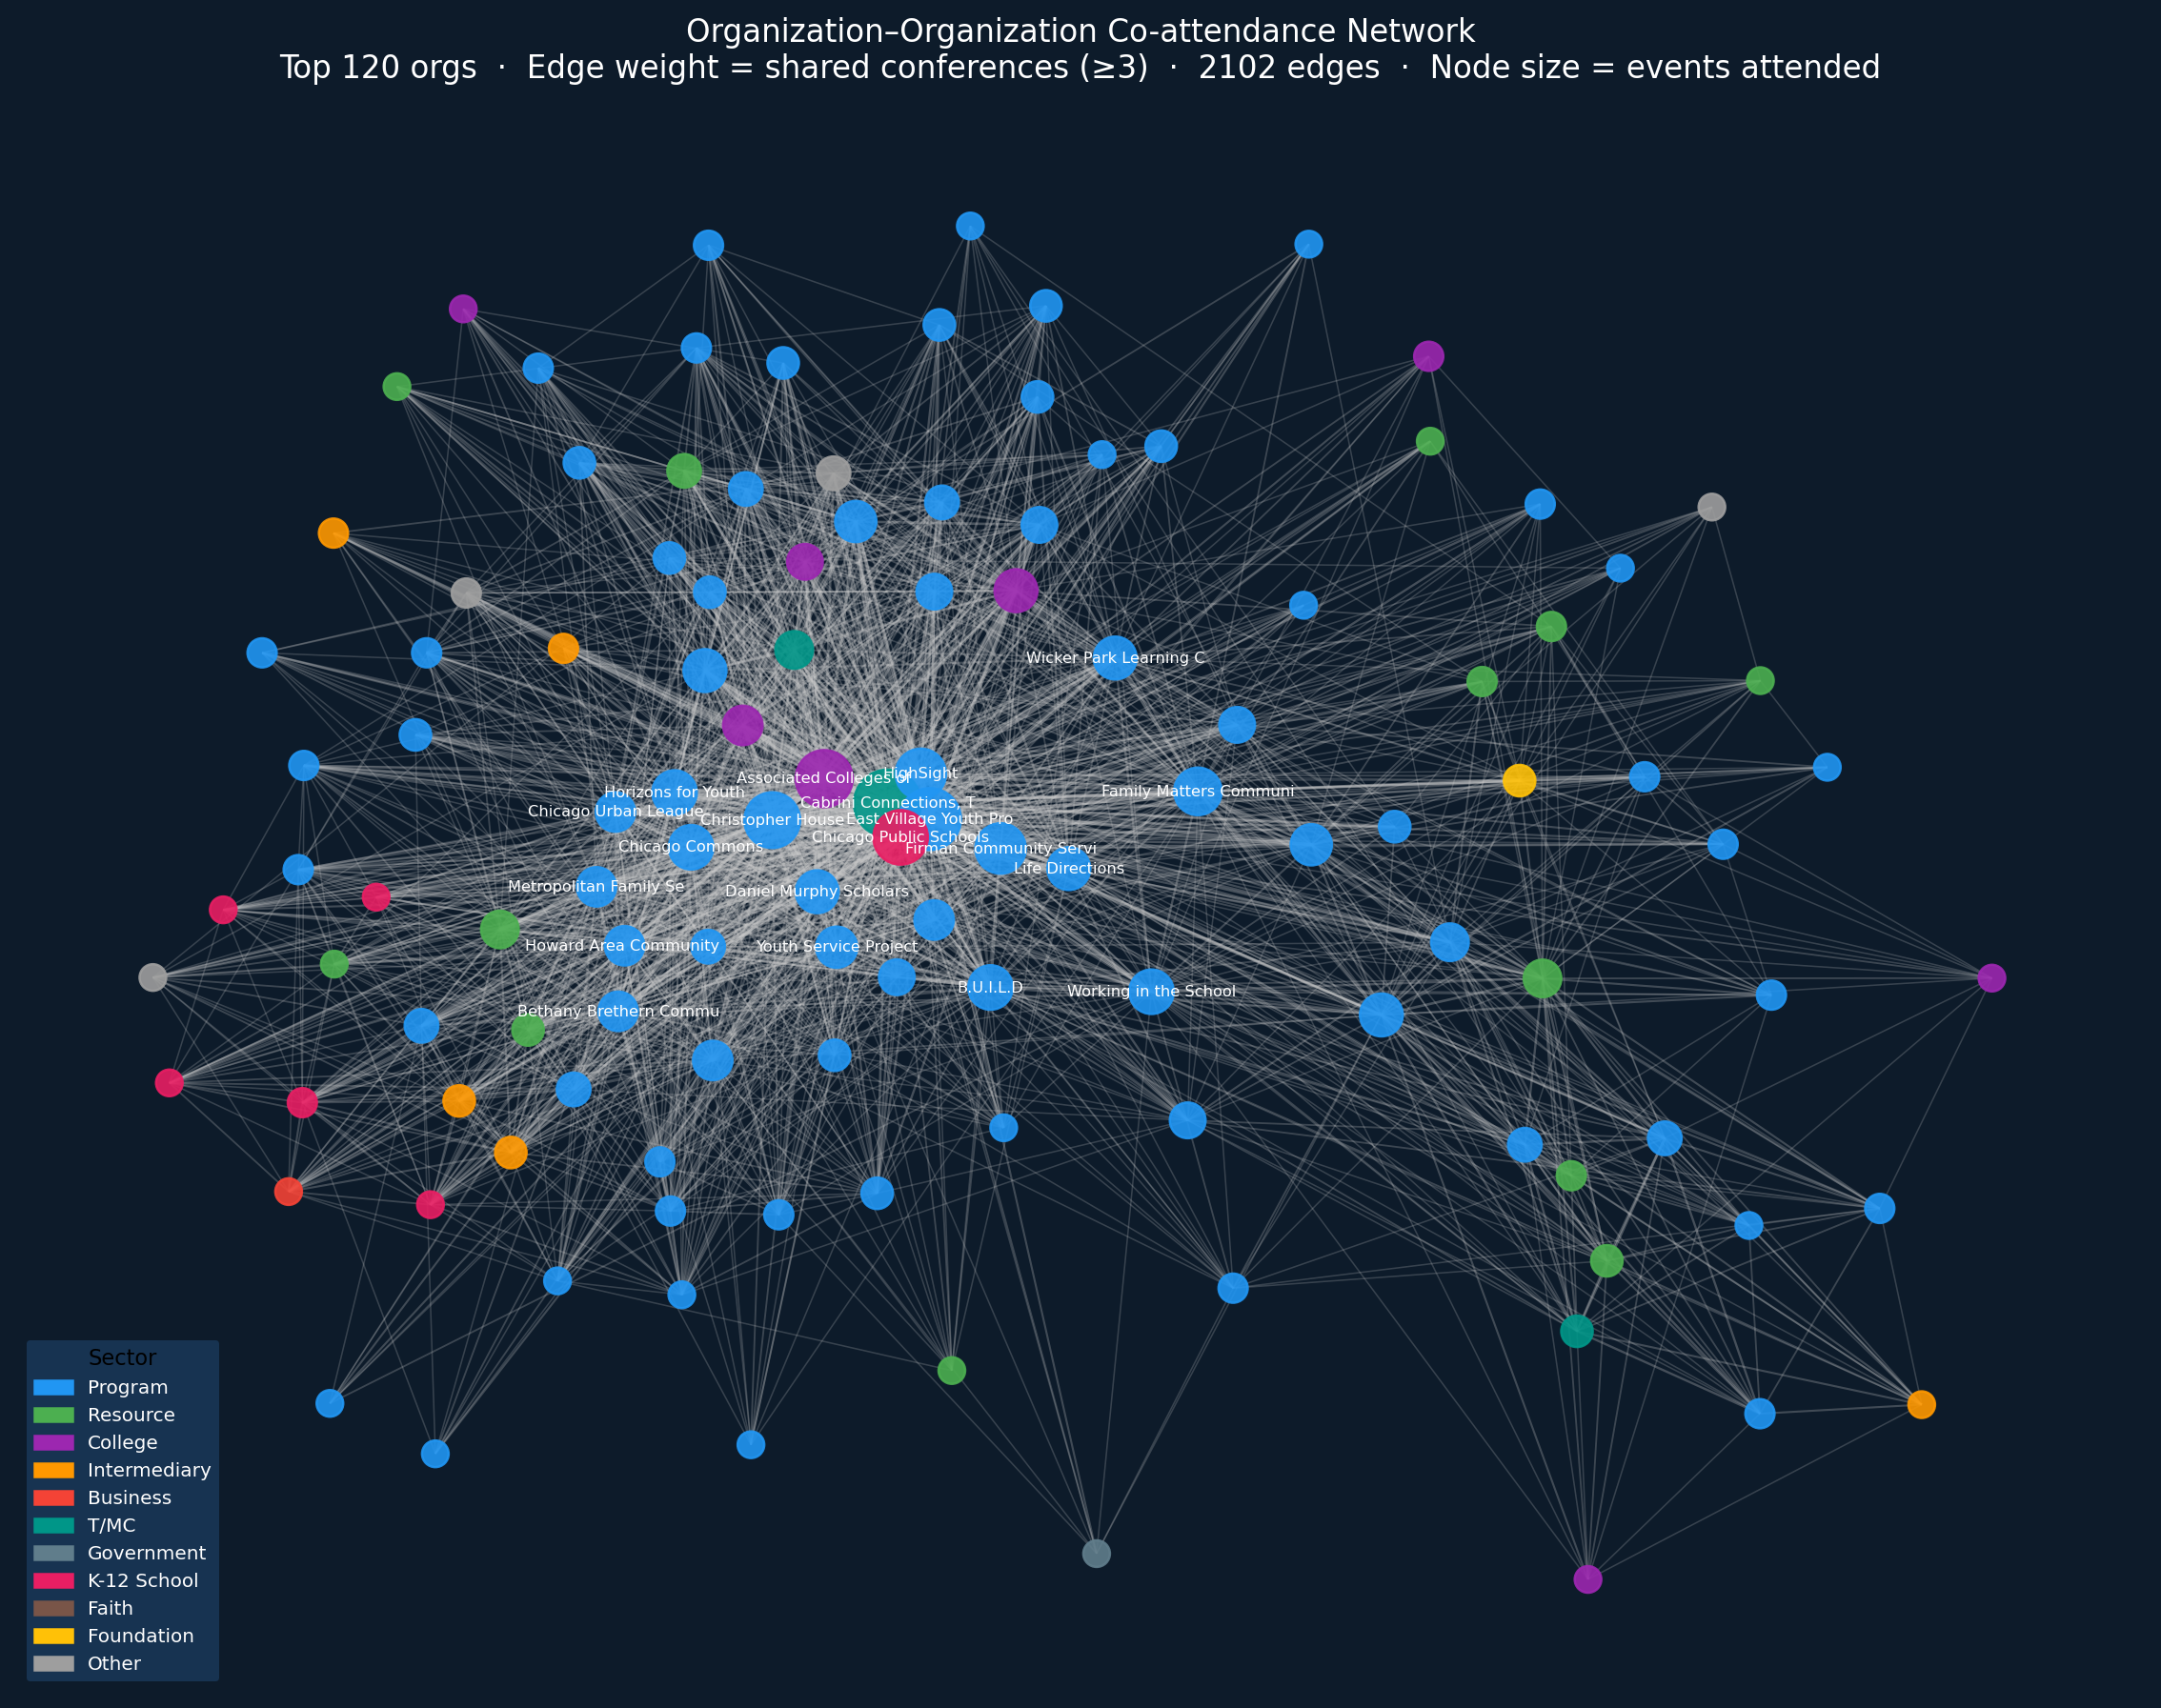
\includegraphics[width=\columnwidth]{../MappingAndAnalyzingParticipation/network_maps/map2_org_org_coattendance.png}
  \caption{Org-org co-attendance network (Matplotlib/NetworkX).
    Edge weight = shared conferences co-attended.
    Node size = total event count; color = SNA category.
    Dense core = long-tenured bridge organizations.}
  \label{fig:network}
\end{figure}

The co-attendance map (Fig.~\ref{fig:network}) makes the core/periphery
structure visible: a small set of high-betweenness organizations has
bridged multiple sectors over decades, while the periphery is large and
sparse with single-event attendees. Linking this map live in Kumu.io
(rather than embedding a static PNG) lets users filter and zoom to
identify specific bridge organizations for targeted re-engagement.

%-----------------------------------------------------------------------
\section{Validation and Redesign}

The platform was evaluated at two points. \textbf{Client evaluation}:
in an April~22,~2026 working session with Daniel F.\ Bassill, the
team demonstrated the live app and collected structured feedback on
the dashboard, network maps, and the \textit{YourConferenceNetwork}
tool. Key changes that resulted: (a)~Kumu network maps are linked
to live maps rather than embedded as static PNGs, following the
approach used by the previous TeamK; (b)~Media was confirmed as
the 12th SNA category and added in this submission; (c)~a dashboard usage
guide is targeted for the next sprint. \textbf{Peer review}: three
reviewers evaluated the intermediate submission against the course
rubric. Privacy-driven scope decision: individual name search was
removed from the dashboard after a reviewer flagged re-identification
risk. Deliverable scope decision: the fully interactive Kumu export
was deferred to the final sprint rather than shipped incomplete---
better to be transparent about scope than to deliver a partial feature.

%-----------------------------------------------------------------------
\section{Usage and Critique of AI Tools}

\textbf{Claude Code} (Anthropic, \texttt{claude-sonnet-4-6}) was
the primary development tool. It produced the entire Django
codebase---views, models, URL routing, export endpoints,
network-map generation, HTML templates---as well as the org-website
crawler and all \texttt{.tex} documentation. No code was written
manually. Strengths: high-level goal interpretation, self-correction
of runtime errors, automatic design-decision documentation.
Limitations: cannot verify URL-to-organization correctness; manual
spot-checking of org URLs is necessary. All AI output was reviewed
before inclusion in deliverables.

%-----------------------------------------------------------------------
\section{Interpretation of Results}

\textbf{Program-sector dominance.} Program organizations account for
3,310 records (51.6\%)---more than all other sectors combined, and
only revealed clearly after normalization collapsed 69 raw variants.
No other sector exceeds 10\%. This means Bassill's conferences
successfully mobilized service-delivery organizations but consistently
failed to bring in the resource providers---funders, media, and
policy actors---who determine whether those programs survive.

\textbf{Underrepresented sectors and why it matters.}
Foundation (58, 0.9\%), Business (131, 2.0\%), and Faith (148, 2.3\%)
are chronically absent over 21 years. The likely cause is structural
visibility: Bassill described in the April~22 session that he
``never had the visibility to make that happen''---without consistent
institutional sponsorship or a university-backed convening authority,
reaching funders and corporate partners through a grassroots conference
is difficult. Their absence is not noise; it is the central challenge
the visualization makes legible for future partners and institutional
sponsors who could help close the gap.

\textbf{Peak engagement and decline.} Attendance peaked in 1999
(565 records) and stayed above 400 through 2002. After 2009 it fell
sharply: 2010 (138), 2011 (180), 2012 (138), 2013 (226), 2014 (209),
averaging 178 per year---less than a third of the peak. This correlates
with the institutional transition from T/MC to Tutor/Mentor Institute
LLC and the financial pressures of that period. The trend line is an
actionable signal: any strategy aimed at reviving conference attendance
has a clear historical benchmark to measure against.

\textbf{Network core vs.\ periphery.} The co-attendance graph
reveals a dense core of long-tenured bridge organizations whose
high betweenness centrality held the network together across sectors
for decades, and a large periphery of single-event attendees who
never returned. Future work with RapidFuzz-based organization
deduplication and SNA centrality metrics would make the core
organizations identifiable by name for targeted re-engagement outreach.

\textbf{Geographic concentration.} Illinois accounts for 5,305 of
state-coded records. ZIP-code-level choropleth maps---a recommended
next step using the Chicago Data Portal shapefile---would reveal which
neighborhoods were consistently underrepresented, directly informing
outreach planning for Bassill's equity-focused mission.

\textbf{Future roadmap.} Immediate priorities: (1)~join
\texttt{org\_websites.csv} to the database for clickable org
profiles; (2)~add a dashboard usage guide.
Medium-term: replace static PNGs with D3.js or Sigma.js
in-browser graphs; add betweenness and eigenvector centrality
metrics; add geographic ZIP-code maps. Longer-term: integrate OHATS
assessment data as a second Django app layer, enabling combined
conference-attendance $+$ organizational self-assessment analysis
(see \texttt{ProjectFiles/OHATS\_path\_forward.pdf}).

%-----------------------------------------------------------------------
\section*{Acknowledgments}

The team thanks \textbf{Daniel F.\ Bassill} (Tutor/Mentor Institute
LLC) for the dataset, sustained guidance, and the April~22,~2026
working session. We acknowledge Fall~2025 \textbf{TeamK} and the
second Fall~2025 team, whose prior cleaning and template work
form the foundation of this project. We thank the E483/E583
Information Visualization (Spring~2026) instructors and TAs
at Indiana University's Luddy School of Informatics, Computing,
and Engineering.

%-----------------------------------------------------------------------
\begin{thebibliography}{9}

\bibitem{borner2015}
K.\ B\"{o}rner.
\textit{Atlas of Knowledge: Anyone Can Map}.
MIT Press, 2015.

\bibitem{borner2018}
K.\ B\"{o}rner, A.\ Bueckle, and M.\ Ginda.
``Data visualization literacy: Definitions, conceptual frameworks,
exercises, and assessments.''
\textit{PNAS}, 116(6):1857--1864, 2018.

\bibitem{bassill2025}
D.\ F.\ Bassill.
``Mapping \& Analyzing Participation: Using Kumu.io to Visualize
Tutor/Mentor Conference Networks.''
Tutor/Mentor Institute LLC.
\url{https://tutormentorexchange.net/mapping-participation}, 2025.

\bibitem{crawler2026}
B.\ Hanley et al.
``Organization Website Crawler: Methodology, Implementation Notes,
and AI-Assisted Development.''
Mapping and Analyzing Participation Project, April 2026.
\texttt{ProjectFiles/org\_website\_crawler\_writeup.pdf}.

\bibitem{teamk2025}
TeamK (Fall 2025).
``Mapping Event Participation --- Final Report.''
Indiana University E483/E583 Information Visualization, 2025.

\end{thebibliography}

\end{document}
